\documentclass[a4paper,twoside,11pt]{article}
\usepackage{a4wide,graphicx,fancyhdr,amsmath,amssymb}
\usepackage{tikz}
\usepackage{tikz-qtree}
\usetikzlibrary{shapes} 
\usepackage{enumitem}
\usepackage{amsmath}

%----------------------- Macros and Definitions --------------------------

\setlength\headheight{20pt}
\addtolength\topmargin{-10pt}
\addtolength\footskip{20pt}

\newcommand{\N}{\mathbb{N}}
\newcommand{\ch}{\mathcal{CH}}

\newcommand{\solution}[1]{\noindent{\bf Solution to Exercise #1:}}

\fancypagestyle{plain}{%
\fancyhf{}
\fancyhead[LO,RE]{\sffamily\bfseries\large technische universiteit eindhoven}
\fancyhead[RO,LE]{\sffamily\bfseries\large 2IW02 RTSD}
\fancyfoot[LO,RE]{\sffamily\bfseries\large department of mathematics and computer science}
\fancyfoot[RO,LE]{\sffamily\bfseries\thepage}
\renewcommand{\headrulewidth}{0pt}
\renewcommand{\footrulewidth}{0pt}
}

\pagestyle{fancy}
\fancyhf{}
\fancyhead[RO,LE]{\sffamily\bfseries\large technische universiteit eindhoven}
\fancyhead[LO,RE]{\sffamily\bfseries\large 2IW02 RTSD}
\fancyfoot[LO,RE]{\sffamily\bfseries\large department of mathematics and computer science}
\fancyfoot[RO,LE]{\sffamily\bfseries\thepage}
\renewcommand{\headrulewidth}{1pt}
\renewcommand{\footrulewidth}{0pt}

\def\addsquare#1{\tikz\node[draw]{#1};} 

%-------------------------------- Title ----------------------------------

\title{\vspace{-\baselineskip}\sffamily\bfseries Exercise 1}
\author{
	Rick Veens \qquad Studentno: 0912292\\
	\texttt{r.veens@student.tue.nl}
	\and
	Huib Donkers \qquad Studentno: 0769015\\
	\texttt{h.t.donkers@student.tue.nl}
}

\date{\today}

%--------------------------------- Text ----------------------------------

\begin{document}
\maketitle

\section{}
\subsection{}
\subsubsection{}
SystemDF:\\
	\centerline{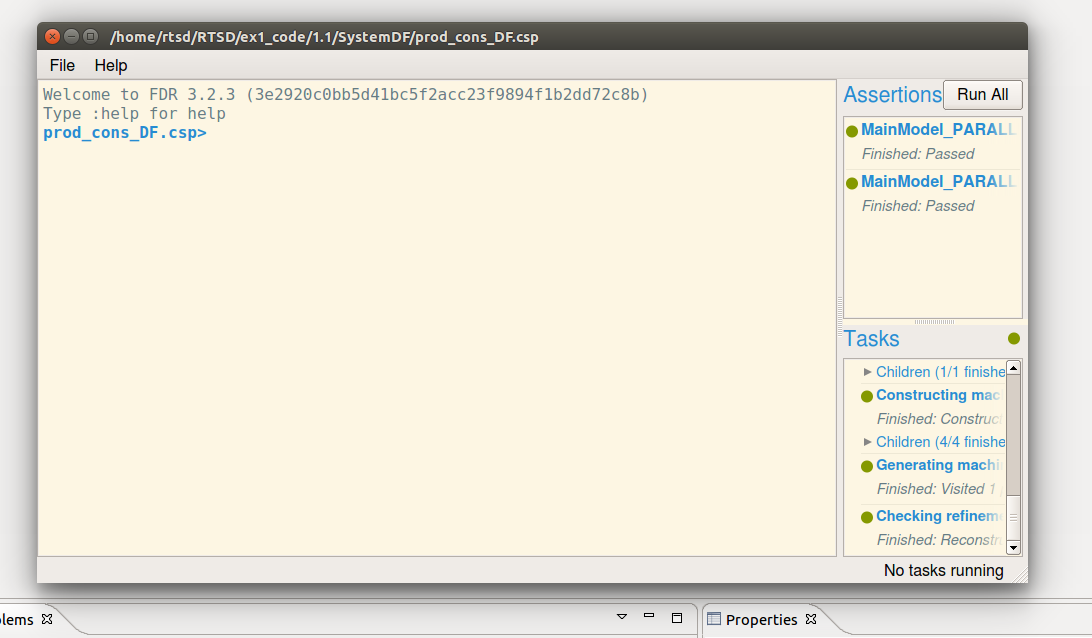
\includegraphics[width=\linewidth]{./images/1_1-SystemDF.png}}
	\centerline{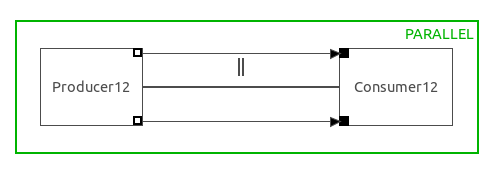
\includegraphics[width=\linewidth]{./images/1_1-SystemDF_main.png}}
	\centerline{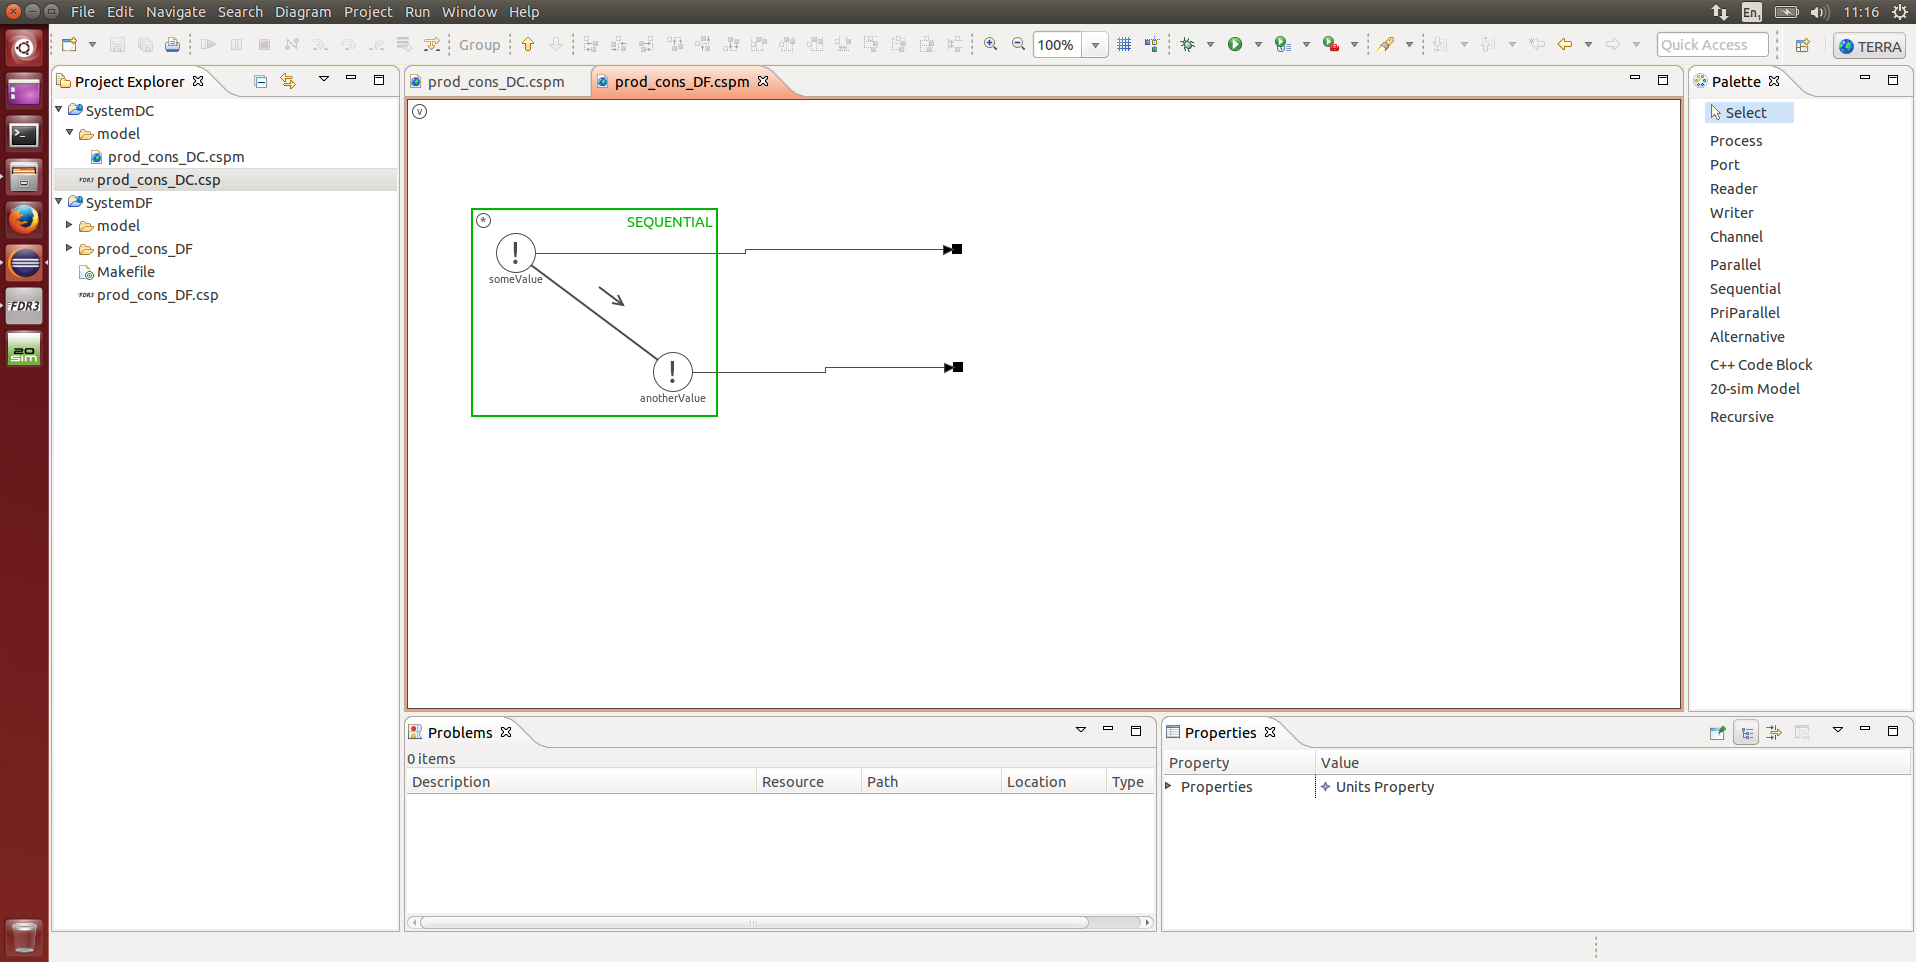
\includegraphics[width=\linewidth]{./images/1_1-SystemDF_cons.png}}
	\centerline{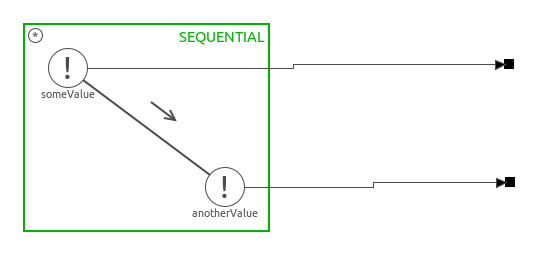
\includegraphics[width=\linewidth]{./images/1_1-SystemDF_prod.png}}

SystemDC:\\
	\centerline{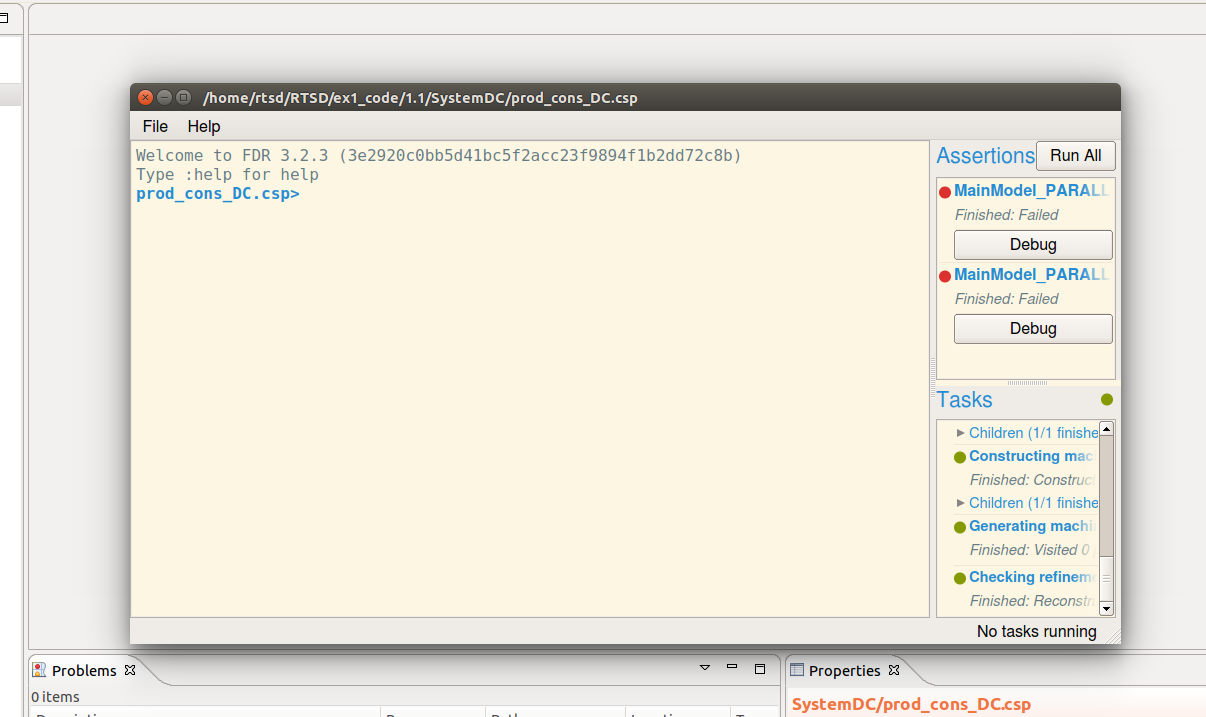
\includegraphics[width=\linewidth]{./images/1_1-SystemDC.png}}
	\centerline{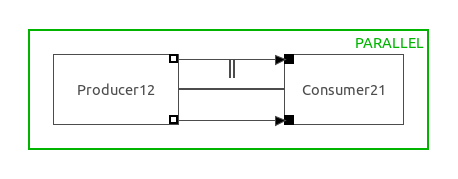
\includegraphics[width=\linewidth]{./images/1_1-SystemDC_main.png}}
	\centerline{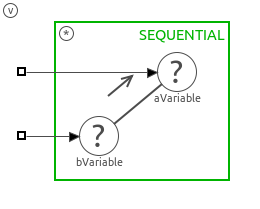
\includegraphics[width=\linewidth]{./images/1_1-SystemDC_cons.png}}
	\centerline{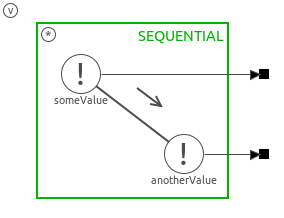
\includegraphics[width=\linewidth]{./images/1_1-SystemDC_prod.png}}
\subsubsection{}
\end{document}
